\section{Logische Gatter}

\subsubsection{Ralisierungsaufwand}
Anzahl Transistoren ist ein m"ogliches Mass f"ur Komplexit"at (Marketing). In der Technik spricht man von Gatter"aquivalent: 1 Gatter"aquivalent entspricht 4 Transistoren.

\subsection{Anzahl Schaltfunktionen}
Permutation: $F= {2^2}^n$ F: Anzahl m"oglicher Schaltfunktionen, n: Anzahl Eing"ange

	\subsection{Verhalten logischer Gatter}
		\begin{multicols}{2}
			\subsubsection{St"orabstand}
				High-Pegel: $ U_{nH} = U_{aHmin} - U_{eHmin} $\\
				Low-Pegel: $ U_{nL} = U_{eLmax} - U_{aLmax} $\\
				
		%\end{multicols}

		%\begin{multicols}{2}
			\subsubsection{Propagation delay Time Anstiegs- bwz. Abstiegszeit}
				Zeit zwischen 50\% von $V_{max}$ am Eingang und 50\% von $V_{max}$ am Ausgang.\\
				$t_{pd}=\frac{t_{pLH}+t{pHL}}{2}$\\
				
			\subsubsection{Transition delay Time (Verz"ogerungszeit)}
				Zeit zwischen 10\% und 90\% von $V_{max}$.\\
				$t_{tLH}$: Transition time low to high.\\
				$t_{tHL}$: Transition time high to low.\\
				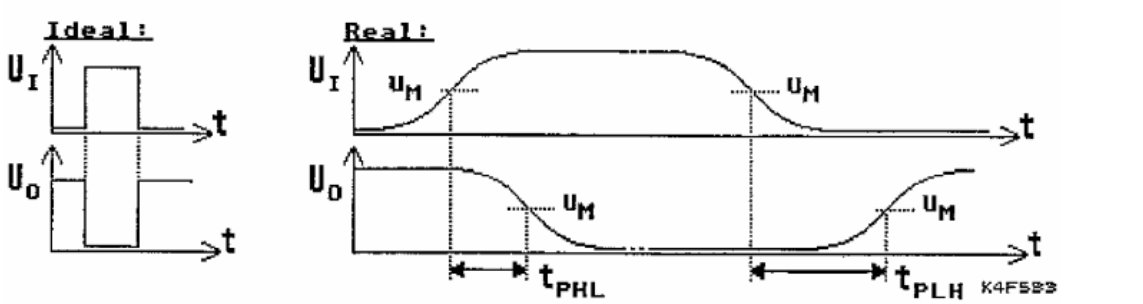
\includegraphics[width=0.2\textwidth]{pics/delay}
				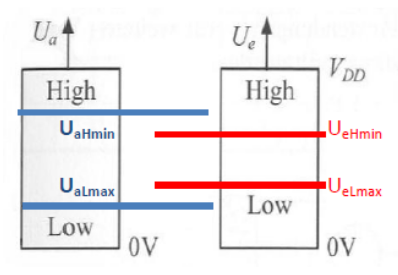
\includegraphics[width=0.2\textwidth]{pics/Pegelbereiche_Stoerabstand}
		\end{multicols}
		
		
\subsection{Aufbau logischer Gatter}

%\newpage
\begin{sidewaystable}
\begin{tabular}{|c|c|c|c|c|c|c|c|c|}
\hline
Funktion & Buffer & NOT & AND & NAND & OR & NOR & EXOR & XNOR\\
& & Nicht & Und & Nicht Und & Oder & Nicht Oder & Exklusiv Oder & Nicht Ex. Oder\\
& & Inverter & Konjunktion & & Disjunktion & & Antivalenz & "Aquivalenz \\
\hline
Formel & a & $ \overline a $ & $ a \cdot b $ & $ \overline{a \cdot b} $ & $ a + b $ & $ \overline{a + b} $ & $ a \oplus b $ & $ \overline{a \oplus b} $\\
& a & $ \overline a $ & $ a \wedge b $ & $ \overline{a \wedge b} $ & $ a \vee b $ & $ \overline{a \vee b} $ & $ a \not= b $ & $ \overline{a \not= b} $ \\
& a & !a & $ a \& b $ & $ !(a \& b) $ & a\#b & !(a\#b) & a\$b & !(a\$b) \\
& & & & & & & $ a \veebar b $ & $ \overline{a \veebar b} $\\
\hline
& & & & & & & &\\
& 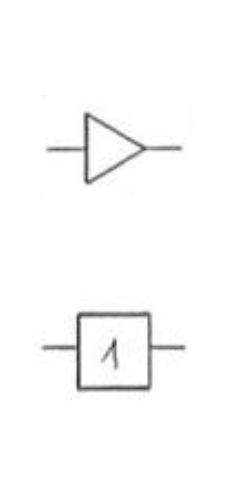
\includegraphics[width=0.08\textwidth]{pics/gates_symbol/buffer} & 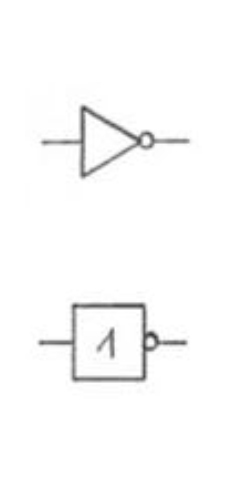
\includegraphics[width=0.08\textwidth]{pics/gates_symbol/not} & 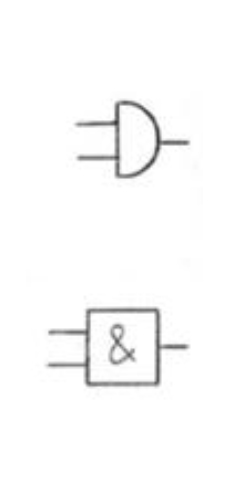
\includegraphics[width=0.08\textwidth]{pics/gates_symbol/and} & 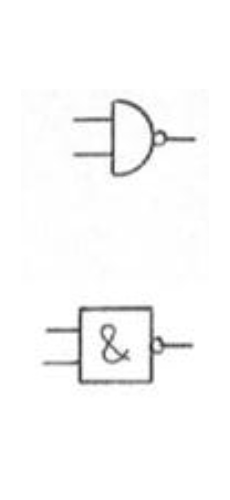
\includegraphics[width=0.08\textwidth]{pics/gates_symbol/nand} & 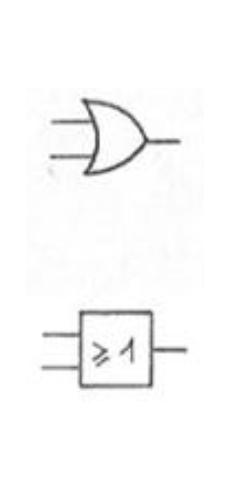
\includegraphics[width=0.08\textwidth]{pics/gates_symbol/or} & 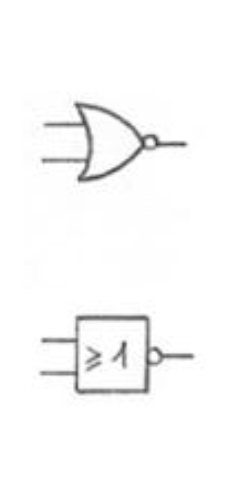
\includegraphics[width=0.08\textwidth]{pics/gates_symbol/nor} & 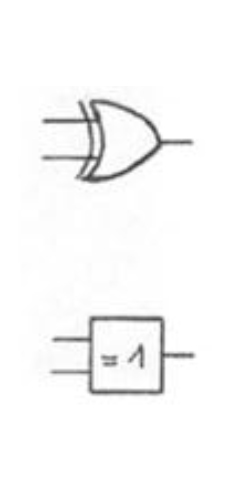
\includegraphics[width=0.08\textwidth]{pics/gates_symbol/exor} & 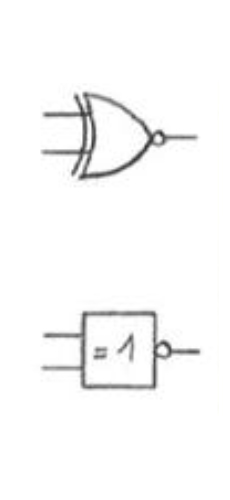
\includegraphics[width=0.08\textwidth]{pics/gates_symbol/xnor} \\
\hline
(0,0) & 0 & 1 & 0 & 1 & 0 & 1 & 0 & 1\\
(0,1) &   &   & 0 & 1 & 1 & 0 & 1 & 0\\
(1,0) & 1 & 0 & 0 & 1 & 1 & 0 & 1 & 0\\
(1,1) &   &   & 1 & 0 & 1 & 0 & 0 & 1\\
\hline
KDNF & \#(1) & \#(0) & \#(3) & \#(0,1,2) & \#(1,2,3) & \#(0) & \#(1,2) & \#(0,3) \\
KKNF & \&(0) & \&(1) & \&(0,1,2) & \&(3) & \&(0) & \&(1,2,3) & \&(0,3) & \&(1,2)\\
\hline
& & & & & & & &\\
& & 
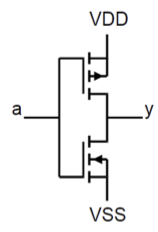
\includegraphics[width=0.12\textwidth]{pics/gates_schematic/inverter} & 
$ \overline{NAND} $ &
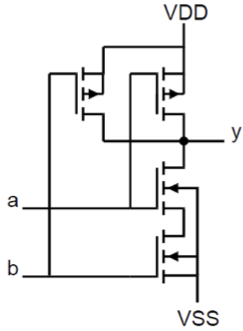
\includegraphics[width=0.12\textwidth]{pics/gates_schematic/NAND} &
$ \overline{NOR} $ &
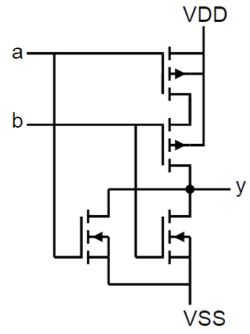
\includegraphics[width=0.12\textwidth]{pics/gates_schematic/NOR} & 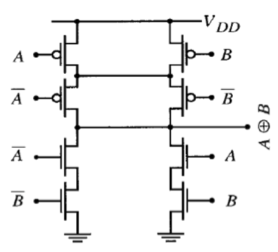
\includegraphics[width=0.12\textwidth]{pics/gates_schematic/XOR} & 
\\
\hline
\#Trans & & 2 & 6 & 4 & 6 & 4 & 8 & \\
\hline
\end{tabular}
\end{sidewaystable}